% verify_plot.tex
% Figure for   I = \iiint_E (1 - x^2 - 2y^2 - 3z^2) dV ,  E : x^2 + 2y^2 + 3z^2 <= 1 .
% Exact value  I = 4*pi*sqrt(6)/45 = 8*pi/(15*sqrt(6)) ~= 0.6840266 .
% Compile with:  lualatex verify_plot.tex  (or pdflatex)
\documentclass[border=6pt]{standalone}
\usepackage{pgfplots}
\pgfplotsset{compat=1.18}
\usepgfplotslibrary{groupplots}
\begin{document}
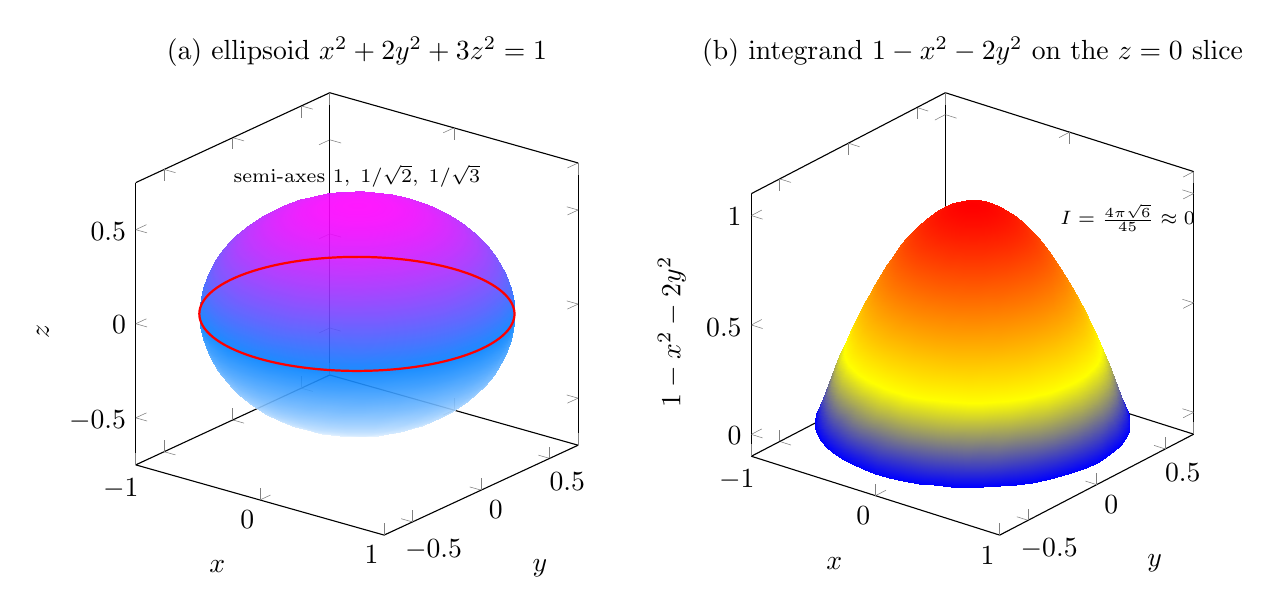
\begin{tikzpicture}
\begin{groupplot}[
    group style={group size=2 by 1, horizontal sep=2.2cm, ylabels at=edge left},
    width=7.2cm, height=7.2cm,
  ]

  % ---------------- (a) the ellipsoid x^2 + 2y^2 + 3z^2 = 1 ----------------
  \nextgroupplot[
      title={(a) ellipsoid $x^2+2y^2+3z^2=1$},
      xlabel=$x$, ylabel=$y$, zlabel=$z$,
      view={38}{22}, colormap/cool,
      zmin=-0.75, zmax=0.75,
    ]
    \addplot3[
        surf, shader=interp, opacity=0.9, z buffer=sort,
        domain=0:360, y domain=0:180, samples=51, samples y=26,
      ]
      ({sin(y)*cos(x)}, {sin(y)*sin(x)/sqrt(2)}, {cos(y)/sqrt(3)});
    % the z = 0 cross-section (the ellipse x^2 + 2y^2 = 1)
    \addplot3[domain=0:360, samples=120, samples y=0, red, thick]
      ({cos(x)}, {sin(x)/sqrt(2)}, {0});
    \node[anchor=south, font=\scriptsize] at (axis cs:0,0,0.62)
      {semi-axes $1,\;1/\sqrt2,\;1/\sqrt3$};

  % ------- (b) integrand 1 - x^2 - 2y^2 over the z = 0 cross-section -------
  \nextgroupplot[
      title={(b) integrand $1-x^2-2y^2$ on the $z=0$ slice},
      xlabel=$x$, ylabel=$y$, zlabel={$1-x^2-2y^2$},
      view={38}{26}, colormap/hot,
    ]
    % parameterise the ellipse by radius r in [0,1] and angle t in [0,360]
    \addplot3[
        surf, shader=interp, z buffer=sort,
        domain=0:1, y domain=0:360, samples=26, samples y=61,
      ]
      ({x*cos(y)}, {x*sin(y)/sqrt(2)}, {1-x^2});
    \node[anchor=south west, font=\scriptsize] at (axis cs:0.85,-0.2,1.05)
      {$I=\frac{4\pi\sqrt6}{45}\approx0.684027$};
\end{groupplot}
\end{tikzpicture}
\end{document}
